\documentclass{article}
\usepackage{fullpage}
\usepackage{amsmath,amsthm,amssymb}
\usepackage{url}
\usepackage{cite}
\usepackage{xcolor,colortbl}
\usepackage{graphicx}
\usepackage{tikz}


\begin{document}
\hfill \textbf{Linear vector representations of time series data}

\hfill Ben Black

\section{Linear vector embeddings}

Word2vec, a set of vector word embedding algorithms, transformed certain areas of natural language processing. It had great success in semantic analysis, for example.\cite{w2v1} Now, researchers, startups, and hobbyists are using this new tool for all sorts of tasks, including automatic classification (CITE!), tracking word usage over time (CITE!), etc. 

The way in which this tool works is as remarkable as its success. The algorithm outputs the weights in a layer of a neural network. These weights are typically considered to be a black box, devoid of any interpretation outside the network. But in this case, they have remarkably natural relative interpretations, in particular the famous $\text{man} - \text{King} = \text{woman} - \text{Queen}$. This remarkable quality sparked a theoretical investigation into its success, which unusually for neural network based models, produced a 

In light of this success, a theoretical investigation into this new tool revealed its close relation Truncated Singular Value Decomposition, a linear algebra technique to compress a large matrix into two smaller matrices. 
\cite{random_walk_pmi}
\cite{NIPS2014_5477}


What all these methods have in common is a single output matrix that converts the layer into a value that represents the distance between two words. 

That is, for the $i,j$th entry of the PMI matrix, you calculate it with $I_i \cdot O^t_j$, where $I$ and is a $n$ by $m$ matrix, and $O$ is an $m$ by $n$ matrix.  So you can get all values of the matrix with $IO$, but without actually ever storing that huge matrix in memory. 


Word2vec is specialized to operate on sparse time series data. We hope to introduce a model that gives vectors with similar sorts of linear algebra properties, but that operates on dense time series data, that is, time series which each time step is a large, dense vector, rather than a sparse unique identifier. We hope that this model will allow non-specialists to use clustering, linear regression and other sorts of fast, well known algorithms that depend on these linear assumptions. 

\section{Non-linear vector embeddings}

Dense data has had vector embeddings for a long time. In particular, generative models for images have used vector embeddings (CITE!). However, the resulting vector does not have the nice linear properties of word2vec, and is unusable without complex non-linear approximation techniques like neural networks.

This work proposes a simple way of generating vector embeddings without a generative network. Instead, it takes a page from word2vec and generates a "closeness" value that signals how temporally far apart two vectors are. 

Now, how is this "closeness" value created and why does it imply the desired linear algebra properties?

The matrix version, each sparse id is assigned a vector for the input and the output, and the distance between the two is the distance between the vectors. 

So in this dense version, there is two non-linear mappings between the dense input and two vectors, 

\section{Implementation concepts}

In the midi converter, it lists chords and creates windows around them. For example, in Mary had a little lamb,

\newcommand{\inwindow}{\cellcolor{red!40}}
\newcommand{\windowcenter}{\cellcolor{red!80}}
\begin{tabular}{|c|c|c|c|c|c|}
	\hline
	\windowcenter $E$ & \inwindow $D$ & \inwindow $C$ & $D$ & $E$ & $E$ \\
	\inwindow $E$ & \windowcenter $D$ & \inwindow $C$ & \inwindow $D$ & $E$ & $E$ \\
	\inwindow $E$ & \inwindow $D$ & \windowcenter $C$ & \inwindow $D$ & \inwindow $E$ & $E$ \\
	 $E$ & \inwindow $D$ & \inwindow $C$ & \windowcenter $D$ & \inwindow $E$ & \inwindow $E$ \\
	\hline
\end{tabular}

Notes within these bounds are considered to be "near" and those not in these bounds are "far". 

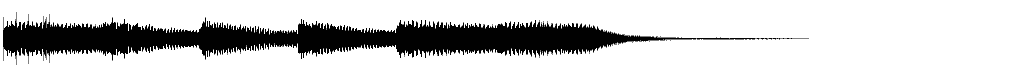
\includegraphics[scale=0.5]{mary_good_waveform.png}


Raw sound does not have predefined notes with discrete values, however, using ffts, it can be divided in a similar way using standard methods. For example, here is the exact same sequence of notes, played by timidity++, a midi sequencer:

\begin{figure}
	\caption{Notes as a modified spectrogram}
	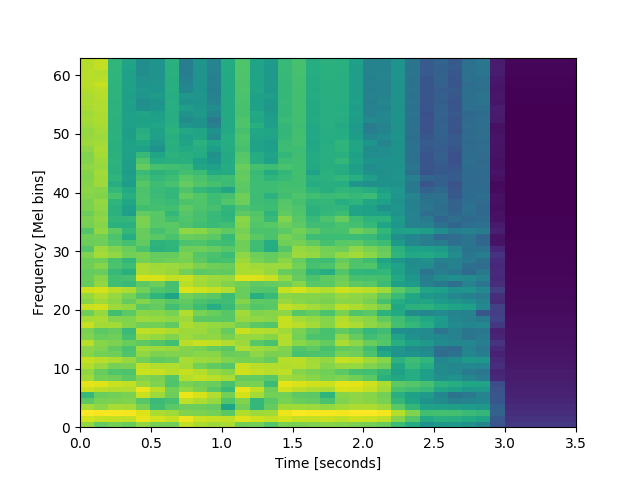
\includegraphics[scale=0.8]{mary_start_plot.png}
\end{figure}

Alt

The song is divided into a smaller number of discrete time chunks. Right now, the implementation creates 10 time chunks per second. 


\section{Time chunk analysis}

The idea is to try to approximate the time series distance function 


% python script to generate table:

%size = 10
%window=2
%
%def t_val(idx):
%return "t"+str(idx+1) 
%
%row1 = " & " + " & ".join(t_val(i) for i in range(size))
%res_list = [row1]
%for x in range(size):
%row_header = t_val(x)
%row = [row_header]
%for y in range(size):
%row.append("1" if abs(y - x) <= 2 else "0")
%res_list.append(" & ".join(row))
%
%res_str = "\\begin{tabular}" + "{" + "|c"*(size+1) + "|" + "}" + "\n"
%res_str += "\\hline \n"
%res_str += "\\\\ \\hline \n".join(res_list)
%res_str += "\\\\ \\hline \n"
%res_str += "\\end{tabular}"
%print(res_str)


\begin{tabular}{|c|c|c|c|c|c|c|c|c|c|c|}
	\hline 
	& t1 & t2 & t3 & t4 & t5 & t6 & t7 & t8 & t9 & t10\\ \hline 
	t1 & 1 & 1 & 1 & 0 & 0 & 0 & 0 & 0 & 0 & 0\\ \hline 
	t2 & 1 & 1 & 1 & 1 & 0 & 0 & 0 & 0 & 0 & 0\\ \hline 
	t3 & 1 & 1 & 1 & 1 & 1 & 0 & 0 & 0 & 0 & 0\\ \hline 
	t4 & 0 & 1 & 1 & 1 & 1 & 1 & 0 & 0 & 0 & 0\\ \hline 
	t5 & 0 & 0 & 1 & 1 & 1 & 1 & 1 & 0 & 0 & 0\\ \hline 
	t6 & 0 & 0 & 0 & 1 & 1 & 1 & 1 & 1 & 0 & 0\\ \hline 
	t7 & 0 & 0 & 0 & 0 & 1 & 1 & 1 & 1 & 1 & 0\\ \hline 
	t8 & 0 & 0 & 0 & 0 & 0 & 1 & 1 & 1 & 1 & 1\\ \hline 
	t9 & 0 & 0 & 0 & 0 & 0 & 0 & 1 & 1 & 1 & 1\\ \hline 
	t10 & 0 & 0 & 0 & 0 & 0 & 0 & 0 & 1 & 1 & 1\\ \hline 
\end{tabular}

However, we will approximate this function using the value of the time series at that time chunk. That is done by transforming the time chunk into a vector, and inputting it into a neural network which is trying to approximate the distance matrix. 

The neural network algorithm looks like this:

With input vectors, $I_1, I_2$, and separate, but identical multi-layer networks 1 and 2, 	

\begin{tikzpicture}[]
\node at (0,8) [draw] (songid) {Song ID};
\draw[step=0.3cm] (2.4,6.0) grid (2.7,10.2)  node[anchor=south] {Song vector};
\draw[thick,->] (1,8) -- (2,8);

\node at (0,2) [draw] (songid) {Song ID};
\draw[step=0.3cm] (2.4,0) grid (2.7,4.2)  node[anchor=south] {Song vector};
\draw[thick,->] (1,2) -- (2,2);
\end{tikzpicture}

%\begin{tikzpicture}[]
%\node at (0,2) [draw]   (ti1) {$I_{t1}$};
%\node at (4,2) [draw]   (tv1) {$V_{t1}$};
%\node at (0,0) [draw]   (ti2) {$I_{t2}$};
%\node at (4,0) [draw]   (tv2) {$V_{t2}$};
%\node at (6,1) [circle, draw]   (dot) {dot};
%\node at (9,1) [draw]   (approx) {Approximate distance};
%
%\path[every node/.style={font=\sffamily\footnotesize}]
%(ti1) [->] edge node [] {Multi-layer-network 1} (tv1)
%(ti2) [->] edge node [] {Multi-layer-network 2} (tv2)
%(tv1) [->] edge node [] {} (dot)
%(tv2) [->] edge node [] {} (dot)
%(dot) [->] edge node [] {} (approx);
%\end{tikzpicture}


The neural network is given the task of approximating the following distance function. 


$l = \sigma(F(x) G(y))$


\bibliography{linearlizer}{}
\bibliographystyle{plain}

\end{document}